\chapter{Lecture}\label{part2:lec14} %%% 14
\markboth{\thechapter. Lecture}{\thechapter. Lecture}

We\pageoriginale were considering the behaviour of $\mathscr{V}_{11}
(\nu /\tau)$ under the general modular transformation:
\begin{equation*}
  \mathscr{V}_{11} \left(\nu \Big/ \frac{a \tau +b}{c \tau+d} \right)=
  C(\tau) e^{\pi i C(c \tau +d)\nu^2} \mathscr{V}_{11} ((c \tau +d)
  \nu /\tau), \tag{1}\label{part2:lec14:eq1} 
\end{equation*}
$a$, $b$, $c$, $d$ integers with $\begin{vmatrix} a & b\\ c &
  d\end{vmatrix} = +1$.

We want to determine $C(\tau)$ as far as possible. We shall do this up
to a $\pm$ sign. $\nu$ is unimportant at the moment; even if we put
$\nu=0$, $C(\tau)$ survives. Put $\nu = \frac{1}{2}, \frac{\tau'}{2},
\frac{1+\tau'}{2}$ in succession, ans use out auxiliary formula which
contracted the whole table into one thing:
\begin{equation*}
  \mathscr{V}_{\mu \nu} \left(v + \frac{k}{2} + \frac{l \tau}{2}\Big/
  \tau\right)= i^{k \mu} e^{-\pi i \tau l^2/4} e^{-\pi i \nu}
  \mathscr{V}_{\mu+l, v+k} (v /\tau)\tag{*}\label{part2:lec14:eq*}
\end{equation*}

Putting $\nu = \frac{1}{2}$ in (\ref{part2:lec14:eq1}), and writing $\tau'= \dfrac{a
  \tau+b}{c\tau+d}$, 
\begin{equation*}
  \mathscr{V}_{11} \left( \frac{1}{2} \Big/ \tau'\right)= C(\tau)
  e^{\pi i c (c \tau+d)/4} \mathscr{V}_{11} \left(\frac{c \tau+d}{2}
  \Big/ \tau\right)\tag{2}\label{part2:lec14:eq2}
\end{equation*}

This is the right moment to call for formula (*). From (*) with
$\nu=0$, $\mu=\nu= 1$, $k=1$, $l=0$, we get 
$$
\mathscr{V}_{11} \left( \frac{1}{2} \Big/ \tau'\right) = i
\mathscr{V}_{12} (0/ \tau')
$$

Also from (*) with $\nu=0$, $\mu=\nu=1$, $k=d$, $l=C$, we get 
$$
\mathscr{V}_{11} \left( \frac{c \tau+d}{2} \Big/ \tau\right)=
i^{d}C^{- \pi i c^2/4} \mathscr{V}_{1+c, 1+d} (o/\tau). 
$$

Substituting\pageoriginale these two formulas in the left and right 
sides of (\ref{part2:lec14:eq2}) respectively, we get 
$$
i \mathscr{V}_{12} (0/ \tau') = C(\tau) e^{\pi i c (c \tau +d)/4}
i^{d} e^{- \pi i \tau c^2/4} \mathscr{V}_{1+c, 1+d} (0/ \tau)
$$

Now, recalling that
\begin{equation*}
  \begin{aligned}
    \mathscr{V}_{\mu, \nu+2} (\nu/\tau) & = \mathscr{V}_{\mu \nu} (\nu/
    \tau)\\
    \mathscr{V}_{\mu+ 2, \nu} (\nu / \tau) & = (-)^\nu
    \mathscr{V}_{\mu \nu} (\nu/\tau),
  \end{aligned}\tag{**}\label{part2:lec14:eq**}
\end{equation*}
the last formula becomes 
\begin{equation*}
  i \mathscr{V}_{10} (0/ \tau') = C(\tau) e^{\pi i cd/4} i^d
  \mathscr{V}_{1+ c, 1+d} (0, \tau) \tag{3}\label{part2:lec14:eq3}
\end{equation*}

Putting $\nu = \tau'/2$ in (\ref{part2:lec14:eq1}), we have 
$$
\mathscr{V}_{11} \left( \frac{\tau'}{2} \Big/ \tau'\right) = C(\tau)
e^{\pi i c/4 \tau'(a\tau+b)} \mathscr{V}_{11}
\left(\frac{a\tau+b}{2}\Big/ \tau\right).
$$

Making use of (\ref{part2:lec14:eq*}) in succession on the left and right sides (with
proper choice of indices) as we did before, this gives 
$$
e^{-\pi i \tau'/4} \mathscr{V}_{12} (0/ \tau') = C(\tau) e^{\pi i c
  \tau' (a \tau +b) /4_i b_e - \pi i a^2
  \tau/4} \mathscr{V}_{1+a, 1+b} (0/\tau),
$$
and this, after slight simplification of the exponents on the right
sides, gives in view of (\ref{part2:lec14:eq**}),
\begin{equation*}
  - \mathscr{V}_{01} (0/\tau') = C(\tau)i^b e^{\pi i ab/4}
  \mathscr{V}_{1+a, 1+b} (0/ \tau) \tag{4}\label{part2:lec14:eq4}
\end{equation*}

Putting\pageoriginale $\nu= (1+ \tau')/2$ in (\ref{part2:lec14:eq1}), 
$$
\mathscr{V}_{11} \left(\frac{1+\tau'}{2} \Big/ \tau'\right) = C(\tau)
e^{\pi i c/4(1+ \tau')(la+c) \tau+ b+d)} \mathscr{V}_{11}
\left(\frac{(a+c)\tau+l+d}{2}\Big/ \tau \right)
$$

Again using (\ref{part2:lec14:eq*}) and (\ref{part2:lec14:eq**}) as we
did earlier, this gives 
$$
i e^{- \pi i \tau' /4} \mathscr{V}_{22} (0/ \tau') = C(\tau)e^{\pi i
  c/4 (1+ \tau')((a+c)\tau+l+d)} i^{l+d} e^{- \pi i (0+ c)^2/4}
\mathscr{V}_{1+a+c, 1+l+d}^{\qquad(0/\tau)}
$$

This of course can be embellished a little:
\begin{align*}
  i \mathscr{V}_{00} (0/ \tau') & = C(\tau) e^{\pi i/4 (1+
    \tau')(c(a+c)\tau + cb+ id+1)} i^{b+d} e^{-\pi i/4} e^{- \pi i
    \tau (a+c)^2/4} \mathscr{V}_{1+a+c, 1+b+d}^{\qquad (0/\tau)}\\
  & = C(\tau) e^{\pi i /4(a+c)((a+c)\tau+b+d)} i^{l+d} e^{- \pi i/4}
  e^{- \pi i \tau (a+c)^2/4} \mathscr{V}_{1+a+c, 1+b+d}\\
  \therefore i \mathscr{V}_{00} (0/ \tau') & = C(\tau) e^{\pi i/4(a+c)
  (b+d)} i^{b+d} e^{-\pi i /4} \mathscr{V}_{1+a+c, 1+b+d}^{\qquad (0/
    \tau)}\tag{5}\label{part2:lec14:eq5} 
\end{align*}

Now utilise the formula:
$$
\mathscr{V}'_1 (0/\tau) = \pi \mathscr{V}_2 (0/ \tau)
\mathscr{V}_3(0/\tau) \mathscr{V}_4 (0/\tau)
$$

Multiplying (\ref{part2:lec14:eq3}), (\ref{part2:lec14:eq4}) and
(\ref{part2:lec14:eq5}), 
\begin{multline*}
  \mathscr{V}_{11}' (0/ \tau') =\ (C(\tau))^3 (-)^{b+d} e^{\pi i/4(ab+cd
    + (a+b)(b+d)-1)}\\ 
  \times i \pi \mathscr{V}_{1+c, 1+d} (0/ \tau)
  \mathscr{V}_{1+a, 1++b} (0/\tau) \mathscr{V}_{1+a+c,
    1+b+d} (0/\tau)
\end{multline*}

Observe\pageoriginale that the sum of the first subscripts on the
right side $=3+2a+2c\equiv 1 \pmod{2}$. So either all three numbers
$1+a$, $1+c$, $1+a+c$ are odd, or one of them is odd and two
even. Then first case is impossible since we should then have both $a$
and $c$ even and so $\big|\begin{smallmatrix} a & b \\ c&
  d \end{smallmatrix}\big|\neq 1$. So two of them are even and one
odd. The even suffixes can be reduced to zero and the odd one to 1 by
repeated application of (\ref{part2:lec14:eq**}). Similarly for the second suffixes. So
the $\mathscr{V}$-factors on the right will be $\mathscr{V}_{00}$,
$\mathscr{V}_{01}$, $\mathscr{V}_{10}$. What we hate is the
combination 1, 1 and this does not occur. (If it did occur we should
have $\mathscr{V}_{11}$ which vanishes at the origin). Although we can
not identify the $\mathscr{V}$-factors on the right, we are sure that
we get exactly the combinations that are desirable: 01, 10, 00. The
dangerous combination is just out.

Let us reduce the subscripts by stages to 0 or 1 as the case may
be. When we reduce the second subscript nothing happens, whereas when
we reduce index by steps of 2, each time a factor $\pm 1$ is
introduced, by virtue of (**). By the time the subscript $1+c$ is
reduced to 0 or 1, a factor $(-)^{\left[\frac{1+c}{2}\right]}(1+d)$
will have accumulated in the case of $\mathscr{V}_{1+c,
  1+d}$. Similarly in the case of $\mathscr{V}_{1+a, 1+b}$ and
$\mathscr{V}_{1+a+c, 1+b+d}$. Altogether therefore
we\pageoriginale have a factor
$$
(-)^{\left[\frac{1+c}{2}\right](1+d)+ \left[\frac{1+a}{2}\right](1+b)
+ \left[\frac{1+a+c}{2}\right](1+b+d)},
$$
and when this compensating factor is introduced we can write
$\mathscr{V}_{00}$, $\mathscr{V}_{11}'$ and $\mathscr{V}_{10}$. Hence
our formula becomes
\begin{equation*}
  \mathscr{V}_{11}' (0 /\tau) = (C(\tau))^3 (-)^\alpha e^{\pi i/4
    (ab+cd+(a+c)(b+d)-1)} i \pi \mathscr{V}_{00} (0 /\tau)
    \mathscr{V}_{01} (0 /\tau) \mathscr{V}_{10}(0/ \tau)
    \tag{6}\label{part2:lec14:eq6} 
\end{equation*}
where
$$
\alpha = b+d + \left[\frac{1+c}{2} \right] (1+d) +
\left[\frac{1+a}{2}\right](1+b)+ \left[\frac{1+a+c}{2}\right] (1+b+d)
$$

From (\ref{part2:lec14:eq1}), differentiating and putting $\nu=0$, we have 
\begin{equation*}
  \mathscr{V}_{11}' (0/\tau')= C(\tau) (C\tau+d) \mathscr{V}_{11}'
  (0/\tau) \tag{7}\label{part2:lec14:eq7} 
\end{equation*}

Dividing (\ref{part2:lec14:eq6}) by (\ref{part2:lec14:eq7}) 
\begin{align*}
  (C(\tau))^2 & = (c \tau +d)(-)^\alpha e^{- \pi i/4
    (ab+cd+(a+c)(b+d)-1)}\\
  & = \frac{c\tau+d}{i} (-)^\alpha e^{- \pi i /4 (ab+cd+(a+c)(b+d)-3)}
\end{align*}
(we may assume $c>0$, since $c=0$ implies $ad =1$ or $a, d= \pm 1$,
which give just translations).
$$
\therefore \quad C(\tau) = \pm \sqrt{\frac{c\tau+d}{i}} i^\alpha
e^{-\pi i/8 (ab+cd+(a+c)(b+d)1-3)}
$$

For the square root we take the principal branch. Since $\im (c
\tau+d)>0$, $\mathscr{R} \dfrac{c \tau +d}{i}> 0$, so that $\dfrac{c
  \tau+d}{i}$ is a point in the right half-plane. The sign is still
uncertain.

The\pageoriginale factor $e^{- \pi i /8 (\cdots)}$ looks like a 16th
root of unity, but is really not so. Since $ad+bc$ has the same parity
as $ad-bc=1$, the exponent is even, and therefore what we really have
is only an 8th root of unity.

What could we do now? We really do not know of any fruitful way. We
cannot copy what we did formerly. There we had a very special case:
$\tau' =- 1/\tau$, or the modular substitution involved was
$\big(\begin{smallmatrix} a & b\\ c& d\end{smallmatrix}\big)=
  \big(\begin{smallmatrix} 0 & -1\\ 1& 0\end{smallmatrix}\big)$. The
    $\pm$ sign depends only on $a$, $b$, $c$, $d$, not on $\tau$, so
    that it is enough if we make a special choice of $\tau$ in the
    equation. Formerly we could take $\tau= \tau'=i$ and it worked so
    beautifully because $\tau$ is a study the fixed points of the
    transformation $\tau'= \dfrac{a \tau +b}{c \tau+d}$. The fixed
    points $\xi$ are given by
$$
\displaylines{\hfill \xi= \frac{a \xi+b}{c \xi+d}, \hfill \cr
  \text{or} \hfill c \xi^2 + (d-a) \xi - b=0 \hfill \cr
  \text{i.e.,} \hfill \xi = \frac{(a-d)\pm \sqrt{(a-d^2)+ 4bc}}{2c} \hfill
  \cr
  \hfill \quad = \frac{(a-d)\pm \sqrt{(a+d)^2-4}}{2} \hfill }
$$
since $ad-bc=1$.

Hence we have several possibilities. If the square root is imaginary we
have twp points one in each of the upper and lower half-planes,
and\pageoriginale for this $|a+d|<2$, so that the square root
becomes $\sqrt{-4}$ or $\sqrt{-3}$ according as $|a+d|=0$or 1. This
is the \textit{elliptic case}. If $|a+d|=2$, we have one rational
fixed point; this is the \textit{parabolic case}. And in the huge
infinity of cases, $|a+d|>2$, we have two real fixed points -the
\textit{hyperbolic} case. Here the fixed are not accessible to us
because they are quadratic algebraic numbers on the real axis.

In the elliptic case with $|a+d|<2$ we could finish the thing without
much trouble. In the parabolic case we are already in a fix. Much more
difficult is the hyperbolic case.

\medskip
\noindent
\begin{minipage}[c]{4.5cm}
\qquad  If $\xi_1$ and $\xi_2$ are the fixed points, $\tau$ and $\tau'$ will
lie on the same circle through $\xi_1$ and $\xi_2$, and repetitions of
the transformation would give a sequence of points on the same circle
which may converge to either $\xi_1$ or $\xi_2$. So the ambiguity in
the $\pm$ sign will remain.
\end{minipage}
\begin{minipage}[c]{5.5cm}
  \begin{figure}[H]
    \centering{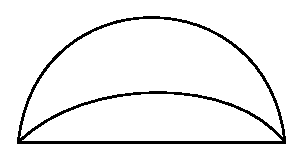
\includegraphics{vol2-figures/fig2.19.eps}}
  \end{figure}
\end{minipage}

It will be much more difficult when we pass from $\mathscr{V}$ to
$\eta$, because then we shall have to determine a cube root.


